%%%%%%%%%%%%%%%%%%%%%%%%%%%%%%%%%%%%%%%%%
% University Assignment Title Page 
% LaTeX Template
% Version 1.0 (27/12/12)
%
% This template has been downloaded from:
% http://www.LaTeXTemplates.com
%
% Original author:
% WikiBooks (http://en.wikibooks.org/wiki/LaTeX/Title_Creation)
%
% License:
% CC BY-NC-SA 3.0 (http://creativecommons.org/licenses/by-nc-sa/3.0/)
% 
% Instructions for using this template:
% This title page is capable of being compiled as is. This is not useful for 
% including it in another document. To do this, you have two options: 
%
% 1) Copy/paste everything between \begin{document} and \end{document} 
% starting at \begin{titlepage} and paste this into another LaTeX file where you 
% want your title page.
% OR
% 2) Remove everything outside the \begin{titlepage} and \end{titlepage} and 
% move this file to the same directory as the LaTeX file you wish to add it to. 
% Then add \input{./title_page_1.tex} to your LaTeX file where you want your
% title page.
%
%%%%%%%%%%%%%%%%%%%%%%%%%%%%%%%%%%%%%%%%%
%\title{Title page with logo}
%----------------------------------------------------------------------------------------
%	PACKAGES AND OTHER DOCUMENT CONFIGURATIONS
%----------------------------------------------------------------------------------------

\documentclass[12pt]{article}
\usepackage[english]{babel}
\usepackage[utf8x]{inputenc}
\usepackage{amsmath}
\usepackage{graphicx}
\usepackage[colorinlistoftodos]{todonotes}
\usepackage{subcaption}

\begin{document}

\begin{titlepage}

\newcommand{\HRule}{\rule{\linewidth}{0.5mm}} % Defines a new command for the horizontal lines, change thickness here

\center % Center everything on the page
 
%----------------------------------------------------------------------------------------
%	HEADING SECTIONS
%----------------------------------------------------------------------------------------

% Name of your university/college
\textsc{\LARGE Instituto Superior T\'{e}cnico}\\[1.5cm]
% Major heading such as course name
\textsc{\Large ISR}\\[0.5cm]
% First Minor heading such as course title
\textsc{\large Report}\\[0.25cm]
% Second Minor heading such as course title
\textsc{\small State Of The Art Milestone}\\[0.25cm]

%----------------------------------------------------------------------------------------
%	TITLE SECTION
%----------------------------------------------------------------------------------------

\HRule \\[0.5cm]
{ \large \bfseries State Of The Art Essay: User Interface Related Work}\\[0.25cm] % Title of your document
\HRule \\[0.5cm]
 
%----------------------------------------------------------------------------------------
%	AUTHOR SECTION
%----------------------------------------------------------------------------------------

\begin{minipage}{0.4\textwidth}
\begin{flushleft} \large
\emph{Author:}\\
Francisco Maria \textsc{Calisto} % Your name
\end{flushleft}
\end{minipage}
~
\begin{minipage}{0.4\textwidth}
\begin{flushright} \large
\emph{Coordinator:} \\
Jacinto \textsc{Peixoto} % Coordinator's Name
\end{flushright}
~
\begin{flushright} \large
\emph{Co-Coordinator:} \\
Daniel \textsc{Gon\c{c}alves} % Co-Coordinator's Name
\end{flushright}
\end{minipage}\\[2cm]

% If you don't want a supervisor, uncomment the two lines below and remove the section above
%\Large \emph{Author:}\\
%John \textsc{Smith}\\[3cm] % Your name

%----------------------------------------------------------------------------------------
%	DATE SECTION
%----------------------------------------------------------------------------------------

{\large 19/04/2016}\\[1cm] % Date, change the \today to a set date if you want to be precise

%----------------------------------------------------------------------------------------
%	LOGO SECTION
%----------------------------------------------------------------------------------------

% 
\includegraphics{ist-logo.png}\\[0.5cm] % Include a department/university logo - this will require the graphicx package

% 
\includegraphics{isr-logo.png}\\[0.5cm] % Include a department/university logo - this will require the graphicx package

\begin{figure}
\centering
\begin{subfigure}{.5\textwidth}
  \centering
  
\includegraphics[width=.5\linewidth]{isr-logo.png}
\end{subfigure}%
\begin{subfigure}{.5\textwidth}
  \centering
  
\includegraphics[width=.5\linewidth]{inesc-id-logo.png}
\end{subfigure}
\begin{subfigure}{.5\textwidth}
  \centering
  
\includegraphics[width=.25\linewidth]{ist-logo.png}
\end{subfigure}
\end{figure}
 
%----------------------------------------------------------------------------------------

\vfill % Fill the rest of the page with whitespace

\end{titlepage}

\section{Abstract}

This paper belongs to Medical Imaging Multimodality Breast Cancer Diagnosis User Interface (MIMBCD-UI) state of the art project stage, describing the related work of Clinical User Interfaces.

\section{Introduction}

Doctors are accountable for decisions they make on behalf of their patients. Likewise, Computer Interface Developers and Engineers must assume accountability for limitations, assumptions and other unplanned deficiencies that impact on the integrity, validity, quantity and timeliness of data made accessible through their interfaces.

Art and science [10] of clinical care are based on an unusual combination of non-judgement trust and exasperating mistrust [1]. Doctors and Clinicians require that theirs patients keep no secrets or else an opportunity to reach the right diagnosis or select the proper therapy may be lost. At the same time, doctors and clinicians are taught to question everything they hear from both colleagues and patients. It is deeply ingrained in medical training to make no important decisions based on information supplied solely by others. The highly trained mistrust explains why many times patients complained that a dozen different people asked the same question. A deeply ingrained aversion incorporate the concept of visual accountability extends well beyond medical user interfaces.

The growing interest in multimodal interface development is inspired in large part by goals of supporting more flexible, transparent, efficient and powerfully expressive means of human-computer interaction than in the past. Multimodal interfaces are expected to support a wider range of diverse applications, be usable by a broader spectrum of the average population, and function more reliably under realistic and challenging usage conditions.

\clearpage

% Commands to include a figure:
\begin{figure}[!hbt]
\centering
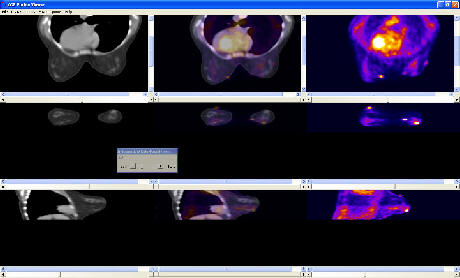
\includegraphics[width=1.00\textwidth]{multimodalbreastimage.png}
\caption{\label{fig:screenshot}A screenshot of a fused data set.
}
\end{figure}

To realise successful multimodal systems of the future, may key research challenges remain to be addressed. Among these challenges are the development of effective natural language processing, dialogue processing, and error-handling techniques. In Addition, new multimodal systems will be needed for collaborative multiperson use. Before this new class os systems can proliferate, toolkits also will be needed to promote software development for both simulated and functioning systems.

Multimodal interfaces also are expected to be easier to learn and use, and they are preferred by users for many applications. They have the potential to expand computing to more challenging applications, be used by a broader spectrum of everyday people, and accommodate more adverse usage conditions than in the past. This class of systems represents a relatively new direction for computing that draws from myriad input and output technologies currently becoming available.

\section{Overview}

Clinical User Interfaces have been extensively discussed in the literature on information visualisation. MIMBCD-UI shows the details of an user interface for diagnosing breast cancer using multimodality medical imaging. MIMBCD-UI have several benefits. In fact, the diagnosis it self is more efficient since the clinical users may navigate using the overview of multimodality of imaging rather than the others techniques. The overview of multimodality of imaging window aids users in keeping track of their current position in the information space [8]. Moreover the overview window itself give users task-relevant information and a feeling of control [9]. A multimodality of views permits to acquire better, more efficient and flexible information and to easily diagnose in it; however, it is more difficult to users to manage information in a more complex user interface.

\section{Related Work}

This section describes existing work in the field of medical and clinical user interfaces.

\subsection{Patient Visualisation}

The Two Different Interfaces to Visualize Patient Histories on a PDA [2] paper describes two different users interfaces for mobile device tool that displays patient histories and permits to visually query patient data stored in hospital database.

\clearpage

% Commands to include a figure:
\begin{figure}[!hbt]
\centering
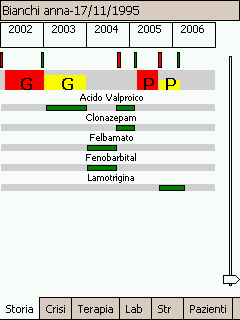
\includegraphics[width=0.50\textwidth]{zoomable.png}
\caption{\label{fig:zoomable}Zoomable interface of PHiP.
}
\end{figure}

The objective of this work is to display as much as possible information about the patient history on a limited display space, providing overview data as well as details. By displaying on a single screen of a personal computer the overview of multiple facets of records will provide users with a better sense of type and volume of available data.

In fact, PHiP (Patient History in Pocket) [2] is a tool designed for a mobile device that displays patient histories and permits to visually query patient data stored in the hospital database exploiting information visualisation techniques where it is able to accommodate on the screen a good amount of clinical cases.

This work has been developed according to an user-centered approach and will bring MIMBCD-UI support in that way. Beside the user studies conducted in the hospital at the requirement phase, they have performed with doctors evaluations of the different prototypes and this kind of information is kindly useful for our research field as well.

\subsection{Usability and Ergonomic Testing}

Semiotic Analysis combined with Usability and Ergonomic Testing for Evaluation of Icons in Medical User Interface [3] research have evaluated the medical icons and iconic interfaces of touch screen ventilator systems used in Intensive Care Unit (ICU).

The use of icons in iconic user interfaces [4] in medical devices like ventilator systems is a common practice. Precise communications through iconic interface between ventilator system and medical users like physicians or nurses is critical to avoid medical errors which may cost patient's life.

This research will help us understand and defining a set of icons that will represent our metaphor analysis throw this work. It also, but not less, give us the right information about usability testing where icons can be tested using various usability testing methods. At last it will help us getting information about Semiotic and Lexical Analysis.

Semiotics is a study of cultural sign processes, analogy, signification, communication, metaphors, signs and symbols [5]. A semiotic analysis is concerned with meaning, which stems from relationships - in particular, the among signs relationships [6].

Linguistics has a term - 'Lexical Analysis' which is the process of converting a sequence of characters into a sequence of tokens. A lexical analysis helped in classification of medical icons [7] into mainly three classes: icons, indices and symbols.

\clearpage

\section{Conclusions}

So far, there have been hardly any specific studies wherein the medical interfaces are tested and evaluated for their comprehensibility and usability to users. Pretty interfaces that hide the ugly reality of underlying data do not engender clinician trust and respect. New visual cues that provide immediate user insight into assumptions and deficiencies regarding the displayed information are required. Clinicians expect and interface to keep clear and direct with easy and intuitive usability.

\clearpage

\begin{thebibliography}{}
\bibitem{} Michael G. Kahn, Janette Coble, and Matthew Orland. 1998. Keep no secrets and tell no lies: computer interfaces in clinical care. In \emph{CHI 98 Cconference Summary on Human Factors in Computing Systems} (CHI '98). ACM, New York, NY, USA, 100-101. DOI=http://dx.doi.org/10.1145/286498.286553
\bibitem{} Carmelo Ardito, Paolo Buono, Maria Francesca Costabile, and Rosa Lanzilotti. 2006. Two different interfaces to visualize patient histories on a PDA. In \emph{Proceedings of the 8th conference on Human-computer interaction with mobile devices and services} (MobileHCI '06). ACM, New York, NY, USA, 37-40. DOI=http://dx.doi.org/10.1145/1152215.1152223
\bibitem{} Ganesh Bhutkar, Ravi Poovaiah, Dinesh Katre, and Shekhar Karmarkar. 2011. Semiotic analysis combined with usability and ergonomic testing for evaluation of icons in medical user interface. In \emph{Proceedings of the 3rd International Conference on Human Computer Interaction} (IndiaHCI '11). ACM, New York, NY, USA, 57-67. DOI=http://dx.doi.org/10.1145/2407796.2407804
\bibitem{} Katre Dinesh. 2004. Experimenting with Uniface: A Tool for
Usability Testing of Icons. \emph{National Usability Conference} (ACM-SIGCHI-SI). Easy 2004, Bangalore, India.
\bibitem{} \emph{http://en.wikipedia.org/wiki/Semiotics\#Terminology} retrieved
on 2nd Nov. 2010.
\bibitem{} \emph{http://www.uk.sagepub.com/upmdata/5171\_Berger\_Final\_Pages\_Chapter\_1.pdf} retrieved on 18th Oct. 2010.
\bibitem{} Poovaiah Ravi. 1995. Graphic Symbols for Environmental
Signage: A Design Perspective. \emph{International Symposium on
Public Graphics}, The Netherlands.
\bibitem{} Plaisant, C., Carr, D., and Shneiderman, B. Image browsers:
Taxonomy, guidelines, and informal specifications. \emph{IEEE
Software, 12(2)}, 1995, 21-32.
\bibitem{} Shneiderman, B. Designing the User Interface. \emph{AddisonWesley},
Reading, MA:1998.
\bibitem{} Daniel Cukier and Joseph W. Yoder. 2011. The artist in the computer scientist: more humanity to our research. In \emph{Proceedings of the 10th SIGPLAN symposium on New ideas, new paradigms, and reflections on programming and software} (Onward! 2011). ACM, New York, NY, USA, 129-136. DOI=http://dx.doi.org/10.1145/2089131.2089134
\end{thebibliography}
\end{document}
